\documentclass{article}
\usepackage[a4paper,left=2cm,right=2cm,top=2cm,bottom=2cm]{geometry}
\usepackage[utf8]{inputenc}  
\usepackage[T1]{fontenc}
\usepackage[french]{babel}
\usepackage{amsmath}
\usepackage{amsfonts}
\usepackage{adjustbox}
\usepackage{dsfont}
\usepackage{graphicx}
\usepackage{caption}
\usepackage{listings}
\usepackage{float}
\usepackage{svg}
\usepackage{diagbox}
\setsvg{inkscapeexe={"D:/Programmes/Inkscape/bin/inkscape.com"}}
\usepackage{pdfpages}
\usepackage{algorithmic}
\usepackage[hidelinks]{hyperref}
\setlength{\parindent}{0pt}
\setlength{\parskip}{1ex plus 0.5ex minus 0.2ex}
\newcommand{\hsp}{\hspace{20pt}}
\newcommand{\HRule}{\rule{\linewidth}{0.5mm}}
\newcommand*{\logeq}{\ratio\Leftrightarrow}

\title{Classement de chiffres manuscrits - Algorithme des K-moyennes et Classification Ascendante Hiérarchique}
\author{Timothé Rios}
\date{mai 2021}

\begin{document}
\maketitle
\newpage
\tableofcontents
\newpage
 

\section{Algorithme des K-moyennes}
\subsection{Apprentissage}
\paragraph{}Afin de faire un premier clustering, on se propose d'effectuer dix fois l'algorithme des K-moyennes et de retenir le clustering ayant la plus petite erreur quadratique.
\subsubsection{Erreur de quantification}
\begin{figure}[h]
\centering
\includesvg[width = \textwidth]{erreur_quadratique(10)}
 \caption{erreur de quantification au fil des itérations des dix initialisations de K-moyennes}
\end{figure}
\paragraph{}On remarque que les erreurs quadratiques initiales et finales de l'algorithme des K-moyennes peuvent varier significativement en fonction de son initialisation.
\subsubsection{Histogramme des classes}
\paragraph{}Le clustering est donc composé de dix classes contenant chacune un certain nombre de données. Dans la figure suivante, chaque graphe correspond à une classe créée par le clustering. Les barres indiquent le nombre d'occurrences d'un même chiffre dans cette classe et le chiffre en bas à gauche du graphe indique le chiffre majoritaire de la classe et donc son label.
\begin{figure}[H]
    \centering
    \makebox[\textwidth][c]{        
    \adjustbox{trim = 0cm 3cm 0cm 2cm}{\includesvg[width = 1.4\textwidth]{hist_cluster(10)}}}
    \caption{histogramme du nombre de chiffres de chaque classe}
    \label{fig:hist_10}
\end{figure}
\paragraph{}On remarque que la plupart des classes ne contiennent qu'un seul chiffre ou presque : 0,2,4,5,6,7 et 8 sont bien différenciés par l'algorithme. Cependant, les trois chiffres restants, 1, 3 et 9, sont confondus par l'algorithme à tel point qu'il n'y a même pas de classe labellisée 9, à cause de la deuxième classe labellisée 1.
L'algorithme a donc eu du mal a différencier 1 et 3 et 3 et 9.
\subsubsection{Indice de la Silhouette}
\begin{figure}[H]
    \centering
    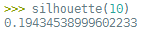
\includegraphics{silhouette(10).PNG}
    \caption{Indice de la Silhouette pour K = 10}
\end{figure}
\paragraph{}L'indice de la Silhouette de ce clustering est positif, ce qui signifie qu'en moyenne, chaque point est plus proche des points de sa classe que de ceux des autres classes. Le clustering est donc efficace.
\subsubsection{Variation du nombre de clusters}
Afin de considérer le meilleur clustering possible pour chaque valeur de K, nous effectuons pour chaque K mille fois l'algorithme des K-moyennes et ne gardons que celui ayant la plus petite erreur de quantification.
\paragraph{}
\begin{figure}[H]
    \centering
    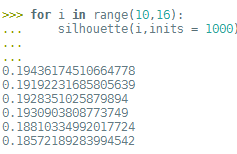
\includegraphics[scale = 0.8]{silhouette(10_15).PNG}
    \caption{Indices de la Silhouette de K=10 à K=15}
\end{figure}
La valeur de K ayant le plus grand indice de la Silhouette est 10. Cependant, il est important de noter que les problèmes de confusion remarqués dans la figure \ref{fig:hist_10} sont grandement réduits avec une valeur de K égale ou supérieure à 14.
\begin{figure}[H]
    \centering
    \makebox[\textwidth][c]{        
    \adjustbox{trim = 0cm 0cm 0cm 0.5cm}{\includesvg[width = 1.1\textwidth]{hist_cluster(15)}}}
    \caption{histogramme du nombre de chiffres de chaque classe (\textit{K = 15})}
\end{figure}
\paragraph{}Par exemple, pour K=15, il ne reste qu'une légère confusion entre 9 et 5 et tous les chiffres labellisent au moins une classe.
\subsection{Classification de la base de test}
\paragraph{}Étant donné que le clustering pour K=10 a donné le meilleur indice de la Silhouette, il a été gardé pour la classification de la base de test.\\
Le clustering à K=15 a aussi été utilisé pour sa réduction des confusions.
\subsubsection{Matrice de confusions}
\begin{figure}[H]
    \centering
    \begin{tabular}{|c|c|c|c|c|c|c|c|c|c|}
        \hline
        176 & 0 & 0 & 0 & 2 & 0 & 0 & 0 & 0 & 0 \\
        \hline
        0 & 156 & 21 & 1 & 0 & 1 & 2 & 0 & 0 & 0\\
        \hline
        1 & 5 & 150 & 9 & 0 & 0 & 0 & 4 & 8 & 0\\
        \hline
        0 & 1 & 0 & 164 & 0 & 2 & 0 & 10 & 6 & 0\\
        \hline
        0 & 9 & 0 & 0 & 160 & 0 & 0 & 7 & 5 & 0\\
        \hline
        0 & 1 & 0 & 31 & 1 & 148 & 1 & 0 & 0 & 0\\
        \hline
        1 & 4 & 0 & 0 & 0 & 0 & 175 & 0 & 1 & 0 \\
        \hline
        0 & 8 & 0 & 0 & 1 & 0 & 0 & 167 & 3 & 0 \\
        \hline
        0 & 28 & 1 & 10 & 0 & 1 & 1 & 1 & 132 & 0 \\
        \hline
        0 & 24 & 0 & 145 & 0 & 4 & 0 & 4 & 3 & 0 \\
        \hline
    \end{tabular}
    \caption{Matrice de confusions pour K=10}    
\end{figure}
\paragraph{}Comme on s'y attendait, aucune donnée représentant le chiffre neuf n'a été classifiée comme neuf, étant donné que le clustering à K=10 ne produit pas de classe labellisée 9. On retrouve donc logiquement les confusions déjà observées à la dixième ligne de la matrice, où l'on s'aperçoit que les données représentant le chiffre 9 se sont vues attribuer en majorité le label 3, puis le label 1.
\begin{figure}[H]
    \centering
    \begin{tabular}{|c|c|c|c|c|c|c|c|c|c|}
        \hline
        177 & 0 & 0 & 0 & 1 & 0 & 0 & 0 & 0 & 0 \\
        \hline
        0 & 153 & 22 & 1 & 0 & 1 & 2 & 0 & 0 & 3\\
        \hline
        1 & 5 & 162 & 0 & 0 & 0 & 0 & 3 & 6 & 0\\
        \hline
        0 & 1 & 2 & 154 & 0 & 2 & 0 & 8 & 5 & 11\\
        \hline
        0 & 5 & 0 & 0 & 171 & 0 & 0 & 5 & 0 & 0\\
        \hline
        0 & 0 & 0 & 0 & 2 & 141 & 1 & 0 & 0 & 38\\
        \hline
        1 & 3 & 0 & 0 & 1 & 0 & 175 & 0 & 1 & 0 \\
        \hline
        0 & 0 & 0 & 0 & 1 & 0 & 0 & 168 & 0 & 10 \\
        \hline
        0 & 19 & 1 & 1 & 0 & 1 & 1 & 1 & 137 & 13 \\
        \hline
        0 & 2 & 0 & 3 & 0 & 2 & 0 & 3 & 2 & 168 \\
        \hline 
    \end{tabular}
    \caption{Matrice de confusions pour K=15}    
\end{figure}
\paragraph{}Par contre, dans le cas du clustering à K=15, on remarque que la quasi-totalité des 9 ont bien été classés. Ainsi, malgré un indice de la Silhouette inférieur, l'algorithme des K-moyennes à K=15 présente de meilleurs résultats que celui à K=10. En contrepartie, le nombre de clusters dépasse le nombre de classes réel.
\section{Classification Ascendante Hiérarchique}
    \subsection{Apprentissage}
    \paragraph{}\paragraph{}Pour notre second clustering, nous faisons un clustering hiérarchique en classification ascendante en utilisant la distance de Ward.
    \begin{figure}[H]
        \centering
        \includesvg[width = \textwidth]{dendrogram_h()}
         \caption{Dendrogramme avec dix clusters visualisés, CAH Ward}
        \end{figure}
        \subsubsection{Histogramme des classes}
        \begin{figure}[H]
            \centering
            \makebox[\textwidth][c]{        
            \adjustbox{trim = 0cm 3cm 0cm 0cm}{\includesvg[width = 1.4\textwidth]{hist_cluster_h(10)}}}
            \caption{histogramme du nombre de chiffres de chaque classe, CAH Ward}
        \end{figure}
        \paragraph{}Contrairement à la méthode des K-moyennes pour K=10, chaque classe s'est vue ici attribuée un label différent et tous les chiffre sont donc représentés. Cependant, la CAH montre plus de confusions. On retrouve les confusions entre  1 et 3 et 3 et 9, comme avec l'algorithmes des K-moyennes, mais la CAH confond en plus 1, 4 et 9. Donc, même si tous les chiffres sont représentés dans les labels des classes, les confusions ne sont pas pour autant moins importantes.
        \subsubsection{Indice de la Silhouette}
        \begin{figure}[H]
            \centering
            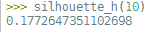
\includegraphics{silhouette_h(10).PNG}
            \caption{Indice de la Silhouette pour 10 clusters, CAH Ward}
        \end{figure}
        \paragraph{}L'indice de la Silhouette de ce clustering est positif, tout comme celui de la méthode des K-moyennes. Les deux valeurs sont d'ailleurs très proches. On note cependant que l'indice de la Silhouette de la méthode des K-moyennes est légèrement meilleur que celui de la CAH.
        \subsubsection{Variation du nombre de clusters}
        \begin{figure}[H]
            \centering
            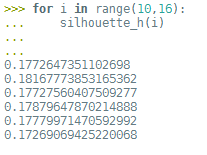
\includegraphics{silhouette_h(10_15).PNG}
            \caption{Indice de la Silhouette pour 10 à 15 clusters, CAH Ward}
        \end{figure}
        \paragraph{}Contrairement à l'algorithme des K-moyennes, l'indice de la Silhouette de la CAH est maximum pour onze clusters. Néanmoins, ce maximum est toujours en dessous de celui obtenu avec la méthode des K-moyennes.
    \subsection{Classification de la base de test}
    \subsubsection{Matrice de confusion}
    \begin{figure}[H]
        \centering
        \begin{tabular}{|c|c|c|c|c|c|c|c|c|c|}
            \hline
            176 & 0 & 0 & 0 & 2 & 0 & 0 & 0 & 0 & 0 \\
            \hline
            1 & 105 & 24 & 1 & 0 & 1 & 2 & 0 & 0 & 50\\
            \hline
            1 & 3 & 141 & 7 & 0 & 0 & 0 & 2 & 22 & 1\\
            \hline
            0 & 1 & 0 & 162 & 0 & 2 & 0 & 9 & 9 & 0\\
            \hline
            0 & 4 & 0 & 0 & 127 & 0 & 3 & 3 & 5 & 39\\
            \hline
            0 & 0 & 0 & 13 & 1 & 166 & 1 & 0 & 0 & 1\\
            \hline
            1 & 3 & 0 & 0 & 1 & 1 & 175 & 0 & 0 & 0 \\
            \hline
            0 & 0 & 0 & 0 & 0 & 0 & 0 & 156 & 2 & 21 \\
            \hline
            0 & 18 & 1 & 4 & 0 & 1 & 1 & 1 & 137 & 11 \\
            \hline
            0 & 0 & 0 & 143 & 0 & 2 & 0 & 3 & 4 & 28 \\
            \hline
        \end{tabular}
        \caption{Matrice de confusions pour dix clusters, CAH}    
    \end{figure}
    \paragraph{}Les confusions apparues dans l'histogramme des classes se retrouvent dans la matrice de confusion : comme pour l'algorithme des K-moyennes, peu de chiffres 9 ont été reconnus comme tel. À la différence de ce dernier, le nombre de 9 reconnus n'est pas nul mais les nombres de 1 et de 4 non reconnus sont beaucoup plus importants.
    \begin{figure}[H]
        \centering
        \begin{tabular}{|c|c|c|c|c|c|c|c|c|c|}
            \hline
            176 & 0 & 0 & 0 & 2 & 0 & 0 & 0 & 0 & 0 \\
            \hline
            0 & 153 & 23 & 1 & 0 & 1 & 2 & 0 & 0 & 2\\
            \hline
            1 & 5 & 142 & 3 & 0 & 0 & 0 & 2 & 21 & 3\\
            \hline
            0 & 1 & 1 & 153 & 0 & 2 & 0 & 6 & 6 & 14\\
            \hline
            0 & 4 & 0 & 0 & 173 & 0 & 1 & 0 & 3 & 0\\
            \hline
            0 & 0 & 0 & 0 & 1 & 163 & 1 & 0 & 0 & 17\\
            \hline
            1 & 3 & 0 & 0 & 1 & 1 & 175 & 0 & 0 & 0 \\
            \hline
            0 & 0 & 0 & 0 & 1 & 0 & 0 & 160 & 2 & 16 \\
            \hline
            0 & 21 & 1 & 1 & 0 & 1 & 1 & 1 & 136 & 12 \\
            \hline
            0 & 2 & 0 & 4 & 0 & 3 & 0 & 0 & 2 & 166 \\
            \hline
        \end{tabular}
        \caption{Matrice de confusions pour quinze clusters, CAH}    
    \end{figure}
    \paragraph{}Comme pour la méthode des K-moyennes, si l'on augmente le nombre de cluster jusqu'à quinze, les plus importantes confusions disparaissent : on voit ici que la grande majorité des chiffres sont maintenant bien classés, avec notamment un bond pour les 9 qui sont passés de 28 à 168 instances bien classées.
\subsection{Comparaison Single Linkage et Linkage de Ward}
\paragraph{}Pour ce dernier type de clustering, nous faisons un clustering avec la méthode CAH en utilisant la distance minimale (\textit{Single Linkage}) : contrairement à la distance de Ward qui définit la distance entre deux clusters comme la distance au carré de leurs barycentres, pondérée par leurs effectifs, la distance minimale définit la distance entre deux clusters comme la plus petite distance mesurée entre deux données appartenant chacune à un cluster différent.
\begin{figure}[H]
    \centering
    \makebox[\textwidth][c]{        
    \adjustbox{trim = 0cm 3cm 0cm 0cm}{\includesvg[width = 1.4\textwidth]{hist_cluster_h_sl(10)}}}
    \caption{histogramme du nombre de chiffres de chaque classe, CAH Single Linkage}
\end{figure}
\paragraph{}Cette méthode a créé un unique mega groupe contenant la quasi totalité des observations. les neuf groupes restant ne contiennent seulement qu'une ou deux observations. Cette méthode n'est donc pas du tout adaptée à notre base de données.
\section{Conclusion : Comparaison des confusions}
\begin{figure}[H]
    \centering
    \begin{tabular}{|l|c|c|c|c|c|c|}
        \hline
       \diagbox{Méthode}{nombre de clusters} & \textbf{10} & \textbf{11} & \textbf{12} & \textbf{13} & \textbf{14} & \textbf{15} \\
        \hline
        K-moyennes & 369 & 233 & 249 & 218 & 202 & 191\\
        \hline
        CAH & 424 & 390 & 261 & 200 & 199 & 193  \\
        \hline
    \end{tabular}
    \caption{Tableau des confusions}    
\end{figure}
\paragraph{}Ce tableau montre le nombre de chiffres mal classés pour chaque algorithme en fonction du nombre de clusters créés. Il apparaît qu'avec un faible nombre de clusters, l'algorithme des K-moyennes est nettement supérieur à la CAH. Cependant, à mesure que l'on augmente le nombre de clusters, l'écart se ressert jusqu'à être insignifiant par rapport aux variations dans les résultats de l'algorithme des K-moyennes (dues à sa nature stochastique). L'algorithme des K-moyennes est donc meilleur avec un faible nombre de clusters mais la CAH est meilleur avec un grand nombre, notamment parce qu'il est déterministe : il suffit d'une seule itération de l'algorithme pour trouver le clustering optimum.
\end{document} 